\documentclass[12pt, letterpaper]{report}
\usepackage{minted}
\usepackage{caption}
\usepackage{tocloft}
\usepackage{acro}
\usepackage{pdfpages}
\usepackage[toc,page,title]{appendix}
\usepackage[colorlinks=true]{hyperref}
\usepackage{graphicx}
\usepackage{gensymb}
\usepackage{amsmath}
\usepackage{mismath}
\usepackage{mathfixs}
\usepackage{pdflscape}
\usepackage{geometry}
\usepackage{csquotes}
\definecolor{usfgreen}{rgb}{0, 0.40, 0.28}
\newcommand*{\sectref}[1]{\hyperref[{#1}]{\ref*{#1}: \nameref*{#1}}}
\newcommand*{\itemref}[1]{\hyperref[{#1}]{\autoref*{#1}}}
\newcommand*{\boxedimage}[1]{\fbox{\includegraphics[width=0.5\textwidth]{img/#1}}}
\newcommand*{\newappendix}[1]{\newpage\section{#1}}
\DeclareCaptionType{codesample}[Code Sample][List of Code Samples]
\DeclareCaptionType{eqn}[Equation][List of Equations]
\newcommand{\fig}[3]{
  \begin{figure}[!htbp]
    \caption{#1}
    \label{#3}
    \centering
    \boxedimage{#2}
  \end{figure}
}
\newcommand{\eq}[3]{
  \begin{eqn}[!htbp]
    #2
    \caption{#1}
    \label{#3}
  \end{eqn}
}
\newcommand*{\descitem}[1]{\item[#1] \hfill \\ }

% class `abbrev': abbreviations:
\DeclareAcronym{omr}{
  short = OMR ,
  long  = Optical mark recognition ,
  class = abbrev
}
\DeclareAcronym{oer}{
  short = OER ,
  long  = Open educational resources ,
  class = abbrev
}
\DeclareAcronym{csv}{
  short = CSV ,
  long  = Comma seperated values [file] ,
  class = abbrev
}

\begin{document}
\hypersetup{linkcolor=usfgreen}
\definecolor{bg}{rgb}{0.95,0.95,0.95}
\frenchspacing

\hyphenation{pro-hib-it-ive-ly Scan-tron ubiq-uit-ous cor-respond-ing Auto-matic}

\acsetup{first-style=short}

\AtBeginEnvironment{appendices}{\renewcommand\thesection{\Alph{section}}}
\renewcommand{\appendixname}{Appendix}

\title{OpenMCR: An Open-Source Tool for OMR Exams}
\author{Ian Sanders\\[1cm]{\small Supervisor: Dr. Autar Kaw, PhD.}}
\date{December 2019}
\maketitle

\tableofcontents
\listofcodesamples
\listoffigures
\listofeqns
\printacronyms[include-classes=abbrev,name=Abbreviations]

\chapter{Introduction}
\section{Background}
Optical mark recognition (\ac{omr}) is a ubiquitous technology whenever large amounts
of controlled physical data needs to be converted to a digital form. This is an
especially common task in the field of education, where the scoring of dozens to
hundreds of multiple choice tests is a regular need. Manual grading of such
examinations is a mundane and time-consuming task that can be easily avoided
with the use of \ac{omr}, as the submission format is completely controlled.
\section{Existing Solutions}
Many of the most popular \ac{omr} solutions presently available are prohibitively
expensive. The most popular product available, sold by Scantron, consists of a
proprietary scanner that is only compatible with Scantron sheets. The scanner
alone can cost several thousand dollars, and the sheets present a continuing
cost for as long as the scanner is in use.

An increasing interest in open educational resources (\ac{oer}) has led to the
development of several free and open source solutions, such as: FormScanner,
queXF, and Auto Multiple Choice. These softwares work extremely well, however,
they have failed to become mainstream due to their increased complexity. Thus,
there exists a need for a simple, free solution that can be implemented with
minimal training or setup time.
\section{Proposed Solution}
A simple, freely available software and mark sheet pair is proposed. By
providing a freely available mark sheet in printable form, setup time is reduced
to the time it takes to download and print the file. In addition, a simple,
easy-to-use software utility that prioritizes reliability will encourage
educators to make the transition from proprietary solutions to an open and free
one. The software will remain simple while still providing a competitive feature
suite and will act as a bridge between raw exam results and more full-featured
exam analysis software.
\subsection{Requirements}
Based on the problem analysis and proposed solution, the final product should:

\begin{enumerate}
  \item Be freely available and open-source
  \item Be as reliable as possible in order to produce fair results
  \item Process files in bulk
  \item Be simple and easy to learn and use
  \item Sort results
  \item Output files that can be input into analysis software
  \item Require minimal setup
  \item Be immediately understood by students taking exams
  \item Provide readily available training resources for educators
  \item Complete processing of results in reasonable amount of time
\end{enumerate}

\chapter{Design of Multiple Choice Sheet}
The multiple-choice sheet is the physical piece of paper that all students
taking exams will fill out. It is also known as a `bubble sheet', easily recognized
by many due to its grid of circles that must be filled in to input answers. In order to
develop a reliable solution with minimal setup, only one sheet is supported
by the software. Therefore, this sheet must be highly optimized.

In order to ensure that the entire solution is freely available to all
educators, an entirely new multiple-choice sheet was developed for use.
This new sheet balances optimization for optical mark recognition with
user-friendliness.

\section{Design Overview}
The optical mark sheet designed for this project consists of several sections,
or `fields'. Several fields provide empty boxes for students to write in their
answers. This provides the administrator with a means to rapidly identify tests
and verify student information. The data fields
also have banded columns to aid users in easily filling in data despite the
larger grids. The completed design is shown in
\itemref{fig:sheet}, while a full printable version is given in \sectref{sect:sheet}.

\fig{Final multiple-choice sheet design.}{sheet.png}{fig:sheet}

The sheet consists of a `student information' section and an `answers' section,
divided by a location for student signatures. The following fields are
included:
\begin{description}
  \descitem{Last Name} For the student's last name. Space for 12 alphabetic
  characters is provided.
  \descitem{First [Name]} For the student's first name. Space for 6 alphabetic
  characters is provided.
  \descitem{Middle [Name]} For the student's middle name. Space for 2 alphabetic
  characters is provided\footnote{It is expected that any students who have a
  middle name will likely have a middle name longer than two characters; this
  is considered acceptable as the middle name is used primarily for sorting.}.
  \descitem{Student ID} For any ID number that identifies students. This could be an
  official institutional ID or simply a number given by the administrator. Space
  for 10 numeric digits is given.
  \descitem{Course ID} For an ID number that identifies the course. Again, this
  could be official per the institution, or a number generated by the
  administrator to identify the course and section. Space for 10 numeric digits
  is given.
  \descitem{Test Form Code} The optional test form code matches exam results with
  their corresponding answer keys. As described in \sectref{sect:scoring}, this can
  be a single character or multiple.
  \descitem{Signature} An informal (unprocessed) field is provided for the exam-
  taker's signature. This does not affect results in any way.
  \descitem{Date} An informal (unprocessed) field is provided for the date. This is
  intended to pair with the Signature field and thus does not affect results
  either.
  \descitem{Answers} The core of the multiple-choice sheet is the set of up to 75
  multiple-choice answers to fill in. The test designer can choose to use
  anywhere from 1 to 75 questions, with answers A-F (or any combination of 2 or
  more of those), as described in \sectref{sect:scoring}.
\end{description}

\section{Features}
Two primary features make the multiple-choice sheet optimal for use with \ac{omr}.

\subsection{Grid System}
In order to ease the mark recognition process, everything on the sheet is aligned
to a grid of $^3/_{16}"$ squares, as can be seen in \itemref{fig:grid}. This
enables the rapid identification of optical marks without the need for complex
and inconsistent shape-finding algorithms, as described in
\sectref{sect:process}. Not only are items aligned to a grid within their own
field, but also on the same grid as every other item on the sheet
\fig{Multiple-choice sheet with grid visible.}{grid.png}{fig:grid}

\subsection{Corner Marks}
A reliable means for establishing the corners of the grid is essential for
reading any data. To this end, an easily-recognized `corner mark' is provided,
with the far corners of each matching perfectly with the grid corners (as shown
in \itemref{fig:corners}). The corner detection process is described in detail
in \sectref{sect:cornerfinding}, but in short, the algorithm first seeks the
\textbf{L}-shaped mark in the top left corner, and then looks for squares of the
expected size and in the expected location to identify the other marks.

As all marks are constructed from
squares of the same size, the expected size of the other three marks can easily
be obtained. Thus, filtering out other square shapes (such as the write-in field
boxes) is simple as they are a different size.

The marks are intentionally dark enough that they will be easily located when
processed with nearly any printer/scanner combination, but they are only 60\%
gray in order to avoid becoming a distraction for exam-takers. Not only could
distractions negatively impact exam scores; they could also attract unwanted
attention that might result in idle doodling or defacing and render
mark recognition impossible.
\fig{Detail view of multiple-choice sheet corner marks.}{corner_marks.png}{fig:corners}



\chapter{Design of \ac{omr} Software}
The software developed to read the multiple-choice sheets is a free, open-source
utility called \textit{OpenMCR}. This tool provides a simple interface to the
complex process of importing, preprocessing, and reading the filled sheets.
\fig{Logo for OpenMCR software utility.}{logo.png}{fig:logo}

Raw results from the software are output in a \ac{csv} file in the form shown 
in \sectref{sect:rawresults}.

\section{User Interface Design}
OpenMCR provides test administrators with a simple, intuitive interface in which
every option is available on a single screen (\itemref{fig:mainscreen}). Use of the software follows a
simple process from the top of the screen to the bottom:
\begin{enumerate}
  \item The user selects a folder to import image files from. All image files
  located directly in the selected folder will be used.
  \item The user chooses, through simple checkboxes, whether or not to convert
  empty answers to the letter \textbf!G! and multiple selected answers to the
  letter \verb!F!. This can aid with postprocessing of results.
  \item~[\textit{Optional}] The user can upload a custom \ac{csv} file to use as an
  answer key. As described in \sectref{sect:scoring}, the user can also create
  keys using the multiple-choice files themselves, or choose not to provide any
  keys at all.
  \item~[\textit{Optional}] The user can upload a rearrangement \ac{csv} file for
  reordering results based on keys. This can aid with postprocessing of results
  as described in \sectref{sect:rearranging}.
  \item The user selects an output folder to save results in.
  \item The user can choose whether or not to sort results --- again by toggling
  a simple checkbox.
\end{enumerate}
\fig{Main input screen of OpenMCR.}{main_screen.png}{fig:mainscreen}

At the bottom of the screen, a \textit{status} section is provided (\itemref{fig:statuses}). Whenever the
user makes a choice or completes a step, the status messages are updated. When
all error messages are resolved (ie, all required steps are completed), the
\textbf{Continue} button is enabled and processing can be started.

\fig{Examples of potential status messages.}{statuses.png}{fig:statuses}

Two additional buttons are also provided:
\begin{description}
  \descitem{Open Sheet} Opens the multiple-choice sheet PDF directly, making it
  simple and easy to print out more sheets.
  \descitem{Open Help} Opens a PDF file with the entire user manual for the
  software, ideally resolving all problems rapidly and efficiently.
\end{description}

When the user presses \textbf{Continue}, a progress bar appears and any error
messages are shown in the status. Upon completion, a success message and \textbf{Close}
button are shown. These are visible in \itemref{fig:progress}.

\fig{OpenMCR status section during (top) and after (bottom) processing.}{progress.png}{fig:progress}

\section{Features}
In addition to the ability to process exam results from images, the software
offers a number of unique features that distinguish it from existing solutions.

\subsection{Automatic Scoring}
\label{sect:scoring}
If the test administrator desires, the program can automatically score and grade
exams and provide the results in an additional \ac{csv} file. This scoring is
performed by comparing results to a `key', which can be provided either by
uploading a CSV file or by including any exams with a last name of
\verb!ZZZZZZZZZZZZ!. If the software encounters any exam with a last name field
of 12 \textbf{Z}s (or an uploaded answer key file), it will score any exams with
a matching Test Form Code by comparing them to that key. In the scores file,
answers are replaced with either a \verb!1! (indicating a correct answer) or
\verb!0! (indicating an incorrect answer), as shown in \sectref{sect:scoredresults}.

Scores are output both as a number of points (counting each answered question
as 1 point) and as a percentage. Any exam-taker's answers after the last answer
filled on the key are discarded. Thus, the answer key file determines the number
of questions in the exam. If scoring is performed but a student writes in an
invalid Test Form Code, their score will be marked as \verb!NO_KEY_FOUND!.

If the user does not elect to convert multiple selected answers to the letter
\verb!G!, the software supports scoring with multiple correct answers. For
example, if the correct answer for a question is both \verb!A! \textit{and} \verb!B!,
the administrator can fill both bubbles on their key sheet and the students'
results will be compared against the value \verb![A|B]!.

All encountered keys will be output in a separate file which has a structure shown in
\sectref{sect:keys}.

\subsection{Rearrangement by Key}
\label{sect:rearranging}
When analyzing exam data, it is generally beneficial to have consistent
question ordering across all results. However, many administrators choose to
shuffle questions to discourage academic dishonesty. Each different exam
arrangement would require a different key and thus need to be analyzed separately.
However, the user provides a file relating each question across all keys, the
software can automatically rearrange the results file, thus outputting a file
that can be analyzed as if all students took exactly the same exam in the same
order. An example of a keys arrangement file is provided in
\sectref{sect:keysarrangement}.

\subsection{Sorting Results}
A common need voiced by educators is the ability to automatically sort results.
Presently, educators will often manually sort the exam papers prior to scanning.
The software handles this with ease, providing an option to automatically sort
results by name. If this option is enabled, the results files will be sorted
primarily by Last Name, then by First Name, and finally by Middle Name (for any
students with identical last and first names). The keys file will be sorted by
Test Form Code.

If the option is left disabled, files will be output in exactly the same order
they are read.

\section{Optical Mark Recognition Process}
\label{sect:process}
The most challenging, and yet the most important, portion of this project was
the development of a reliable process for computationally processing and reading
images to obtain results. It is absolutely crucial that this process produces
reliable and consistent results in order to treat all students fairly. The
process is described in the following subsections, which are provided in order.

\textit{Note}: The examples given in this section rely closely upon the OpenCV
software library. This and all other libraries used are detailed in
\sectref{sect:acknowledgements}. 

\subsection{Image Preprocessing}
Prior to performing any computer vision steps, the image steps through a series
of preprocessing algorithms that dramatically improve results. Not all scans
are made alike, and therefore the preprocessing step is intended to normalize
images and thus improve consistency. All image processing steps in this section
will be demonstrated on the portion of a scanned multiple-choice sheet shown in
\itemref{fig:sample_original}.

\fig{``Student ID'' portion of a sample scanned-multiple choice sheet prior to any processing.}{sample/original.jpg}{fig:sample_original}

\subsubsection{Noise Removal}
It is far easier for the software to distinguish data from scanned images if
they are processed with a high-frequency noise removal filter first (as is the
case with most real-world data). Thus, the images are softened using a Gaussian
blur, which blurs the image by passing a `kernel' over the image and
replacing each pixel with the weighted mean of the pixels in the kernel around
that point. The pixels towards the center are given a higher weight than those
towards the edges. The steepness of this weight change is controlled by the
$\sigma$ value given to the function, as shown in \itemref{eq:gaussian}.

\eq{2D Gaussian distribution function, where $x$ and $y$ are $0$ at the center of the kernel.}{\[ G(x,y)=\frac{1}{2\pi\sigma^2}e^-\frac{x^2+y^2}{2\sigma^2} \]}{eq:gaussian}

As the resolution of input images is completely unknown this software, the $\sigma$
value and kernel size must be dynamically chosen to avoid over-processing small images or
under-processing large ones. For OpenMCR, the $\sigma$ is calculated such that
the value is equal to $\sqrt{2}$ when the smallest image dimension is 2500
pixels, and directly proportional to this value at other dimensions (\itemref{eq:sigma}). This
provides optimal results at the image size that is expected to be
typical based on a review of modern scanners.

\eq{Relationship used to calculate $\sigma$ for Gaussian distribution, where $w$ is the number of pixels along the smaller side of he input image.}{\[ \sigma(w)=w(5.6569\times10^-4) \]}{eq:sigma}

This is represented in code by \itemref{code:noiseremoval}. An example of
the result of this process is shown in \itemref{fig:noiseremoval}.

\fig{Sample portion of scanned sheet after noise removal flter is applied.}{sample/noise_filtered.jpg}{fig:noiseremoval}

\begin{codesample}[!htbp]
  \caption{Gaussian filter-based noise reduction of an input image.}
  \label{code:noiseremoval}
  \begin{minted}[autogobble, bgcolor=bg]{python}
    import cv2 # OpenCV library

    def remove_hf_noise(image):
      smallest_dimension = min(image.shape)
      sigma = smallest_dimension * 5.6569e-4
      # Setting kernel size to (0, 0) indicates that OpenCV
      # should select a size based on sigma.
      result = cv2.GaussianBlur(
        image, (0, 0), sigmaX=sigma, sigmaY=sigma
      )
      return result
  \end{minted}
\end{codesample}

\subsubsection{Thresholding}

After noise removal, the image is thresholded---that is, each
pixel is converted to either pure black or pure white.
Removing the extraneous color and brightness information
makes shapes sharper and simplifies processing by simply
classifying each pixel as dark or light.

Prior to applying the threshold filter, the image is converted to black and
white to reduce pixel information to a brightness value alone. Then, any pixel
with a brightness value below the set threshold is considered to be black, and
all other pixels are white.

After converting the image to black and white, the binary threshold algorithm is
applied as described above. OpenCV provides a built-in flag to enable Otsu's
thresholding algorithm, which automatically picks a threshold value by treating the image
as one with a bimodal distribution of lumosity, and then taking a value that is
approximately between the two peaks to use as the threshold.

The result of applying this process is shown in \itemref{fig:thresholded}, which
was created using approximately the code given in \itemref{code:thresholding}.

\fig{Sample portion of scanned sheet after thresholding is applied.}{sample/thresholded.jpg}{fig:thresholded}

\begin{codesample}[!htbp]
  \caption{Black-and-white conversion and thresholding of an input image.}
  \label{code:thresholding}
  \begin{minted}[autogobble, bgcolor=bg]{python}
    import cv2

    def threshold(image):
      grayscale_image = cv2.cvtColor(image, cv2.COLOR_BGR2GRAY)
      _, result = cv2.threshold(
        grayscale_image, 0, 255,
        cv2.THRESH_BINARY | cv2.THRESH_OTSU
      )
      return result
  \end{minted}
\end{codesample}


\subsection{Corner Detection}
\label{sect:cornerfinding}
After preprocessing filters are applied, the software must locate the document
corners in order to establish the grid. There is no assumption made as to the
rotation or size of the input document---it could, for example, be scanned as
$^1/_4$ of the input image and angled at $45\degree$ from vertical. Therefore,
the algorithm must be robust. The corner-finding algorithm takes the following
steps.

\subsubsection{Edge Finding}
The Canny edge-detection algorithm simply finds all
locations in the image that are borders between light and dark regions, turns
these locations into white pixels, and leaves all other pixels black. This
enables simple location of common shapes.

The results of edge detection as performed in \itemref{code:edgedetecting} is
shown in \itemref{fig:edgedetected}.

\fig{Sample portion of scanned sheet after edge detection.}{sample/edges.jpg}{fig:edgedetected}

The basic edge-detecting algorithm returns
a matrix of pixels with values of either $1$ or $0$. To convert this matrix to
a list of approximated polygons, each defined by a list of coordinates,
OpenCV provides an additional method (also given in \itemref{code:edgedetecting}).

\begin{codesample}[!htbp]
  \caption{Canny edge-detection and polygon establishment performed on an input image.}
  \label{code:edgedetecting}
  \begin{minted}[autogobble, bgcolor=bg]{python}
    import cv2

    def detect_edges(image):
      return cv2.Canny(
        image, 100, 300, L2gradient=True, edges=3
      )

    def detect_polygons(image):
      edges = detect_edges(image)
      return cv2.findContours(
        edges, cv2.RETR_TREE, cv2.CHAIN_APPROX_SIMPLE
      )
  \end{minted}
\end{codesample}

\subsubsection{Establishing the \textbf{L}-Mark}
The mark in the top-left corner of the multiple-choice sheet is intentionally
shaped to be unique among all other polygons in the document in order to make it
identifiable by the software. The mark is distinguishable by the fact that it
has exactly 6 vertices, all angles are (approximately in the case of a scanned
image) $90\degree$, 4 sides are approximately of length $l$ (what we call
the `unit' length) while the other 2 sides are approximately of length $2l$,
and the two longer sides are adjacent. Therefore, the algorithm is defined as:

\begin{enumerate}
  \item For each polygon:
    \begin{enumerate}
      \item If the number of sides is not 6, go to the next polygon.
      \item Calculate the internal angles at each vertex.
      \item If all angles are not within 15\% of $90\degree$, go to the next polygon.
      \item Calculate the length of each side.
      \item Find the longest two sides.
      \item If the longest two sides are not adjacent, go to the next polygon.
      \item Divide the length of the longest two sides by two.
      \item If the four shortest side lengths and the half-lengths of the
        longest sides are not within 15\% of the mean of those values, go to
        the next polygon.
      \item This polygon is the \textbf{L}-mark. Return it and exit the loop.
    \end{enumerate}
  \item If no mark was found, raise an error.
\end{enumerate}

This algorithm is written in Python in \itemref{code:lmark}.

\begin{codesample}[!htbp]
  \caption{Canny edge-detection and polygon establishment performed on an input image.}
  \label{code:lmark}
  \begin{minted}[autogobble, bgcolor=bg]{python}
    import cv2

    def find_l_mark(polygons):
      for polygon in polygons:
        if len(polygon) != 6:
          continue

        angles = calculate_angles(polygon)
        if any(
          [abs(angle - 90) > (0.15 * 90) for angle in angles]
        ):
          continue

        lengths = calculate_lengths(polygon)
        greatest_indexes = find_greatest_indexes(lengths, n=2)
        if(not are_adjacent(lengths, greatest_indexes)):
          continue

        unit_lengths = [
          length if i not in greatest_indexes
          else length / 2 
          for i, length in enumerate(lengths)
        ]
        l = mean(unit_lengths)
        if any(
          [abs(val - l) > (0.15 * l) for val in unit_lengths]
        ):
          continue
        
        return polygon
      raise RuntimeError("Could not find L-mark.")
  \end{minted}
\end{codesample}


\subsubsection{Establishing Other Marks}
Three points are needed to establish a grid across an image.
In order to make the grid as accurate as possible, points that
are as far away from each other as possible are used. Therefore, it is only
necessary to find the bottom-left and bottom-right corner marks after finding
the \textbf{L}-mark. This significantly limits the area of possibilities for where these marks
may be located. Thus, the location, approximate size (side length $l$), and shape
are all known, so locating these marks is made easier.

The algorithm for locating other marks is similar to that for locating the
\textbf{L}-mark.

\begin{enumerate}
  \item For each polygon:
    \begin{enumerate}
      \item If the number of sides is not 4, go to the next polygon.
      \item Calculate the internal angles at each vertex.
      \item If all angles are not within 15\% of $90\degree$, go to the next polygon.
      \item Establish a coordinate system as defined in \itemref{fig:lmarkcoords} (this process is described in \sectref{sect:coordsystem}).
      \item If all of the points are within 15\% of $64l$ (where $l$ is the unit
      length from the \textbf{L}-mark) from the \textbf{L}-mark on the newly established
      $y$-axis \textit{and} all of the points are within that same range size
      around $x$=0 on the newly established system, return the mark as the
      bottom-left mark.
      \item If all of the points are within 15\% of $64l$ from the \textbf{L}-mark on the
      new $y$-axis \textit{and} all of the points are within 15\% of $50l$ from
      the \textbf{L}-mark on the on the new $x$-axis, return the mark as the bottom-
      right mark.
    \end{enumerate}
  \item If either mark couldn't be found, raise an error.
\end{enumerate}

\fig{Coordinate system established on the \textbf{L}-mark to find other marks.}{coords.png}{fig:lmarkcoords}

\subsection{Grid Establishment}
\subsubsection{Establishing the Coordinate Transformation}
\label{sect:coordsystem}
After locating all three marks, a coordinate transformation can be established from the
three points. The top-left point of the \textbf{L}-mark (point $A$) becomes $(0,0)$, the bottom-left
point of the bottom-left square mark (point $B$) becomes ${(0,1)}$, and the bottom-right point of the
bottom-right square (point $C$) becomes $(1,1)$. This transformation is described
mathematically by \itemref{eq:transform} and can be performed using numpy as
shown in \itemref{code:transform} 

\eq{Transformation of bases from the established coordinate system to one defined by three points $A$, $B$, and $C$, such that $P'(A)=(0,0)$, $P'(B)=(0,1)$, $P'(C)=(1,1)$.}{
  \[\mathbf{M}=\left[\begin{matrix}M_1\\M_2\\M_3\\M_4\\M_5\\M_6\\\end{matrix}\right]=\left[\begin{matrix}A_x&A_y&1&0&0&0\\B_x&B_y&1&0&0&0\\C_x&C_y&1&0&0&0\\0&0&0&A_x&A_y&1\\0&0&0&B_x&B_y&1\\0&0&0&C_x&C_y&1\\\end{matrix}\right]^{-1}\left[\begin{matrix}0\\0\\1\\0\\1\\1\\\end{matrix}\right]\]
  \[\mathbf{T}=\left[\begin{matrix}M_1&M_2\\M_4&M_5\\\end{matrix}\right],\vec{R}=\left[\begin{matrix}M_3\\M_6\\\end{matrix}\right]\]
  \[\vec{P}'(\vec{P})=\mathbf{T}\vec{P}+\vec{R}\]
}{eq:transform}

\begin{codesample}[!htbp]
  \caption{Transformation of bases as described by \itemref{eq:transform}. Accepts points as tuples of $(x,y)$ and returns a pair of transformation functions.}
  \label{code:transform}
  \begin{minted}[autogobble, bgcolor=bg]{python}
    import numpy as np

    def create_change_of_basis(A, B, C):
      from_matrix = np.array([[A[0], A[1], 1, 0, 0, 0],
                              [B[0], B[1], 1, 0, 0, 0],
                              [C[0], C[1], 1, 0, 0, 0],
                              [0, 0, 0, A[0], A[1], 1],
                              [0, 0, 0, B[0], B[1], 1],
                              [0, 0, 0, C[0], C[1], 1]],
                            float)
      target_matrix = np.array([[0], [0], [1], [0], [1], [1]],
                              float)

      M = np.matmul(np.linalg.inv(from_matrix), target_matrix)

      T = np.array([[result[0][0], result[1][0]],
                    [result[3][0], result[4][0]]])
      R = np.array([[result[2][0]], [result[5][0]]])

      def to_basis(point):
          point_vector = np.array(
            [[point.x], [point.y]], float
          )
          result = np.matmul(
            transformation_matrix, point_vector
          ) + rotation_matrix
          return (result[0][0], result[1][0])

      def from_basis(point: Point) -> Point:
          point_vector = np.array(
            [[point.x], [point.y]], float
          )
          result = np.matmul(
            np.linalg.inv(transformation_matrix),
            (point_vector - rotation_matrix)
          )
          return (result[0][0], result[1][0])

      return to_basis, from_basis
  \end{minted}
\end{codesample}

\subsubsection{Establishing the Grid}
Once coordinate transformation functions are obtained, establishing the grid
across the page is simple. It is known that there are 36 grid cells across the
page and 48 grid cells down the page. Thus, the grid cell width is $^1/_{36}$, or
0.0278, and the cell height is $^1/_{48}$, or 0.0208, in the new coordinate
system. The grid (along with the cell masks
described in \sectref{sect:mask}) is shown in \itemref{fig:samplegrid}.

\fig{Demonstration of the grid and cell masks on a sample portion of a scanned sheet.}{sample/grid.jpg}{fig:samplegrid}

\subsection{Mark Reading}
\label{sect:reading}

After the grid is established, the location of each mark is known with complete
confidence. At that point, all that is left is to determine whether each mark
is filled in or not.

\subsubsection{Image Dilation}
Image dilation is another preprocessing step, applied after grid establishment
but before mark reading.
In low-resolution images, the combination of Gaussian blurring and thresholding
can result in significant loss of data, even when using a dynamic $\sigma$ for
the Gaussian filter. There is not enough data in the source image to be able to
sacrifice some data for the purpose of noise removal. However, the noise still
must be removed.

The result of this high level of data loss in this scenario, is that bubbles
that are darker already (those with \textbf{W} or \textbf{B} in them) become
indistinguishable from filled bubbles, as the program only considers the
fraction of dark pixels in a circle to determine whether it is filled or not
(see \sectref{sect:reading}).

It is possible, however, to differentiate these
circles by taking advantage of the fact that the circles containing letters are
more irregular (contain less contiguous chunks of dark or light pixels) than the
filled circles. Thus, an algorithm that can expand chunks of light pixels will
reduce the unfilled circles far more than the filled circles, and this is exactly
what an image dilation algorithm is intended to do. A dilation algorithm passes
over the image with a square kernel and replaces each pixel with the maximum value
of the pixels in the kernel around the original pixel.

As the problem is primarily limited to smaller images, all images are dilated
but the kernel size is \textit{not} dynamic - it is always $3\times3$ pixels.
Therefore, it dramatically affects smaller images while having a much smaller
effect on larger images.

The result of this algorithm as applied in \itemref{code:dilation} can be seen
in \itemref{fig:dilated}.

\fig{Sample portion of scanned sheet after dilation is applied.}{sample/dilated.jpg}{fig:dilated}

\begin{codesample}[!htbp]
  \caption{Simple dilation of an input image.}
  \label{code:dilation}
  \begin{minted}[autogobble, bgcolor=bg]{python}
    import cv2
    import numpy as np

    def threshold(image):
      # Creates a 3x3 matrix of 8-bit integers with a value of 1
      kernel = np.ones((3, 3), np.uint8)
      return cv2.dilate(image, kernel, iterations=1)
  \end{minted}
\end{codesample}

\subsubsection{Cell Masking}
\label{sect:mask}
Each grid cell forms a square around the target mark. To each of these cells, a
circular mask is applied in order to remove any extraneous information (such as
the boundary of a bordering rectangle). The diameter of this mask is 75\% of the
entire cell width, as shown in \itemref{fig:samplegrid}.

\subsubsection{Determining Fill Threshold}
The number of black pixels divided by the total number of pixels in the masked
grid cell for a mark is referred to as the `grid cell fill fraction', $k$. Determining
whether a mark is filled or not requires comparing that mark with a threshold
fill fraction, $j$: if $k>j$, then the cell is filled.

The threshold $j$ is a crucial value---if it is too low, the darkest unfilled marks will be
read as filled. If it is too high, the lightest filled marks will not be read.
To this end, $j$ cannot be a static value; it must be dynamically determined for
each sheet.

It can be observed that the filled marks are expected to be significantly darker
than the unfilled marks. Therefore, the optimal value of $j$ is expected to be
between the two marks with the greatest difference in their $k$ value. However,
if a mark's letter and circle are missing (ie, if an exam-taker erased the mark or
it failed to print), then the greatest difference in $k$ could be between the
missing mark and the first non-missing unfilled mark, which would cause nearly
the entire sheet to be read as filled. Thus, the algorithm assumes that less
than 20\% of the marks are filled (an entirely full sheet only has 10.5\% of
marks filled), and thus only looks in the 20\% of the marks that are most full.

Therefore, algorithm works as follows:
\begin{enumerate}
  \item Calculate the fill percent $k$ of all marks
  \item Sort all marks by their $k$ value
  \item Discard the bottom 80\% of the sorted list
  \item Calculate a new set $h$ where $h_i = k_i - k_{i-1}$
  \item Find the index $g$ of the greatest value in $h$
  \item Return the value $(k_g-k_{g-1})/2$
\end{enumerate}

This algorithm is implemented in \itemref{code:fillthreshold}.

\begin{codesample}[!htbp]
  \caption{Determination of mark fill threshold.}
  \label{code:fillthreshold}
  \begin{minted}[autogobble, bgcolor=bg]{python}
    import numpy as np

    def calculate_fill_threshold(mark_fill_percents):
        sorted_fill_percents = np.sort(fill_percents)

        number_to_keep = round(sorted_fill_percents.size / 5)
        last_chunk = sorted_fill_percents[-number_to_keep:]

        differences = [
            last_chunk[i + 1] - last_chunk[i]
            for i in range(last_chunk.size - 1)
        ]
        greatest_difference_index =
          find_greatest_value_index(differences)

        return (
          last_chunk[greatest_difference_index] +
          last_chunk[greatest_difference_index + 1]
        ) / 2
  \end{minted}
\end{codesample}

After calculating this value, all marks are compared to the value, and mark
reading is complete.

\begin{appendices}
\section{Acknowledgements}
\label{sect:acknowledgements}
This project relies on the following freely available tools and libraries:
\begin{enumerate}
  \item Python 3.7: \url{https://www.python.org}
  \item Nullsoft Scriptable Install System (NSIS): \url{https://nsis.sourceforge.io}
  \item Pyright: \url{https://github.com/microsoft/pyright}
  \item OpenCV: \url{https://opencv.org/}
  \item NumPy: \url{https://numpy.org/}
  \item PyInstaller: \url{https://www.pyinstaller.org/}
\end{enumerate}

\newappendix{Licenses}
\label{sect:licenses}

\subsection{Multiple-Choice Sheet}
The multiple-choice sheet distributed with this report is licensed under the
Creative Commons Attribution-NonCommercial-ShareAlike 4.0 International license
(CC BY-NC-SA 4.0). In summary, this means that you are free to distribute and
modify the document so long as you share it under the same license, provide
attribution, and do not use it for commercial purposes.

For the full license terms,
see \url{https://creativecommons.org/licenses/by-nc-sa/4.0/}.

\subsection{Code}
The OpenMCR software and all code samples in this report are licensed under the
GNU General Public License (3.0):
\begin{displayquote}
Copyright (C) 2019 Ian Sanders

This program is free software: you can redistribute it and/or modify
it under the terms of the GNU General Public License as published by
the Free Software Foundation, either version 3 of the License, or
(at your option) any later version.

This program is distributed in the hope that it will be useful,
but WITHOUT ANY WARRANTY; without even the implied warranty of
MERCHANTABILITY or FITNESS FOR A PARTICULAR PURPOSE.  See the
GNU General Public License for more details.
\end{displayquote}

For the full license terms, see
\url{https://www.gnu.org/licenses/gpl-3.0.en.html}.

\subsection{Report}

All other portions of this report are Copyright (C) 2019 Ian Sanders.

\newappendix{Multiple-Choice Sheet}
\label{sect:sheet}
The full printable multiple-choice sheet is available on the next page. See
\sectref{sect:licenses} for the license information for this sheet.
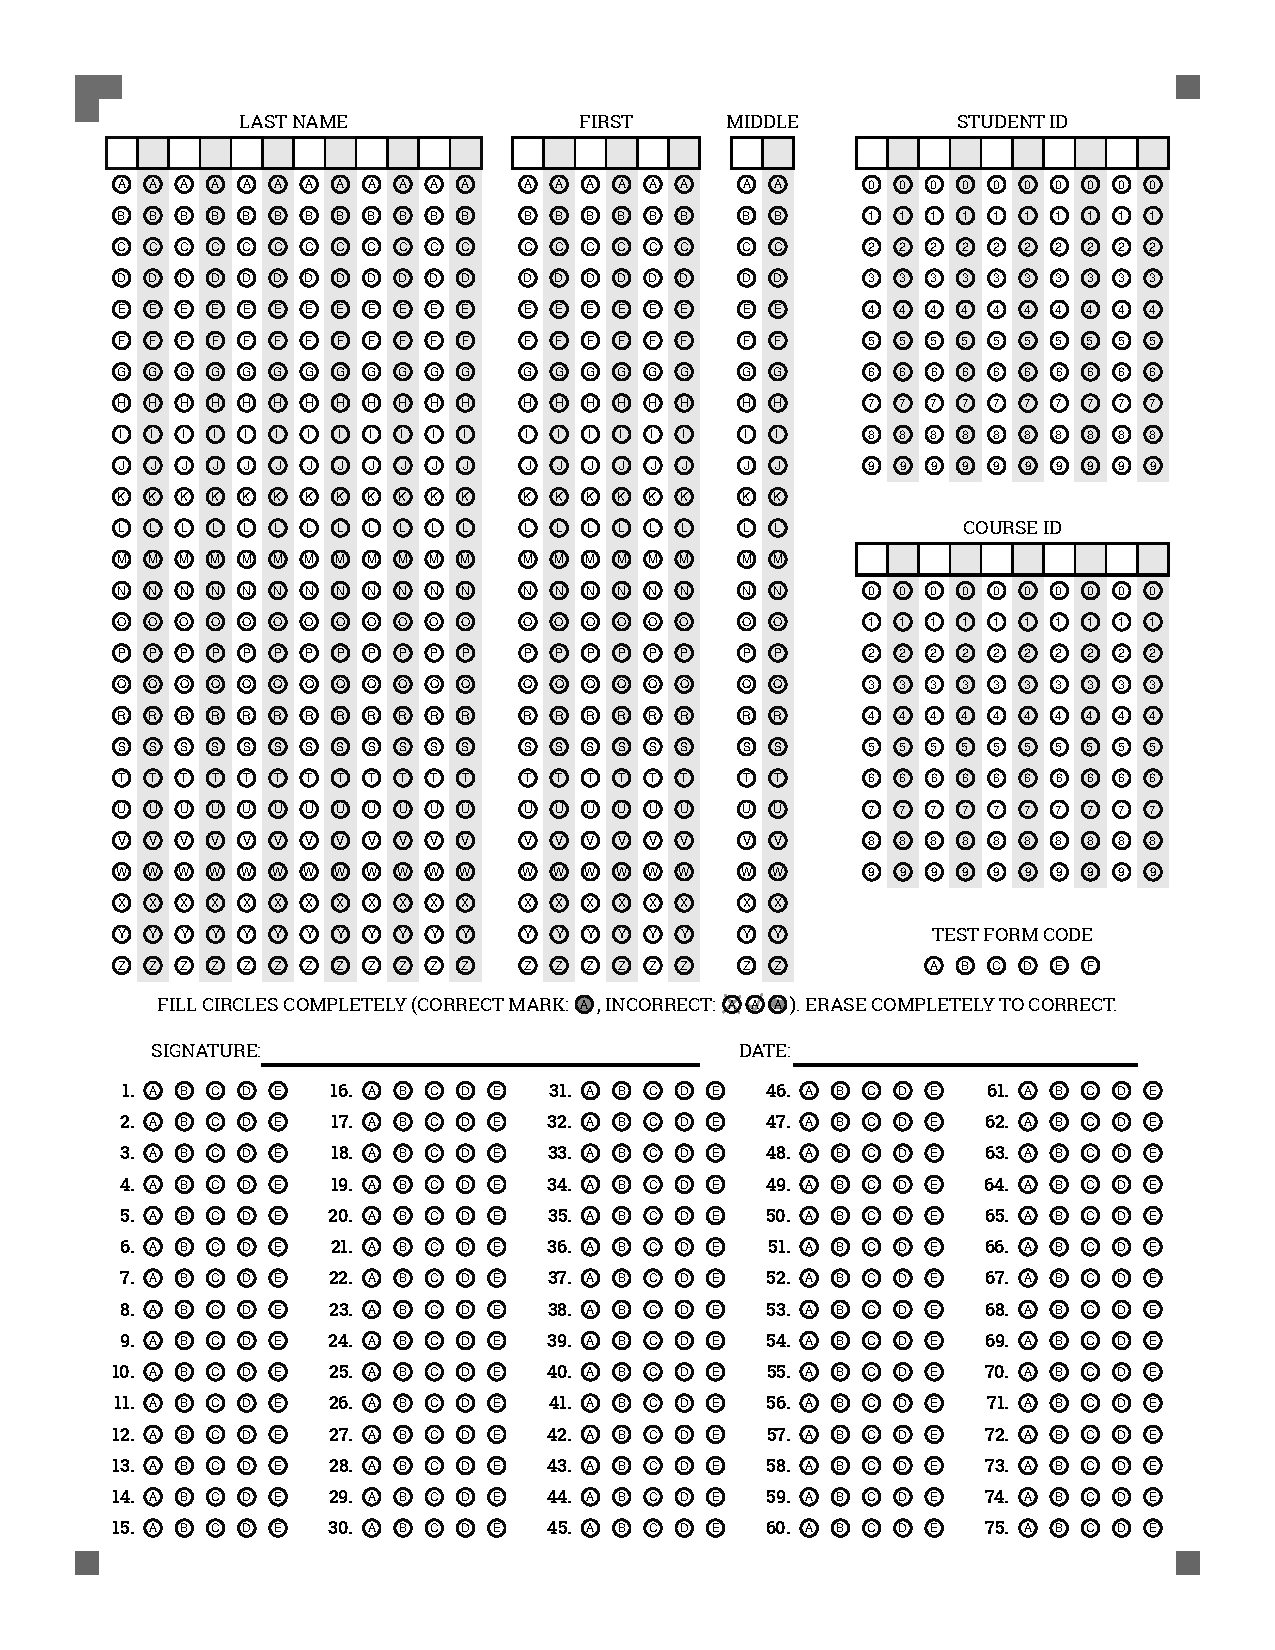
\includepdf{sheet.pdf}

\newappendix{CSV File Structures}
Sample tables representing the CSV file output structures are provided on the
following pages. Note that the CSV file format is a text-based one in which new
table rows are identified by new lines, and columns are delimited by commas.
\newgeometry{bottom=0.5in,left=0.5in}
\begin{landscape}
\subsection{Raw Results}
\label{sect:rawresults}
\verb!YYYY-MM-DD_HH-mm-SS__results.csv!\\
\\
\begin{tabular}{ l | l | l | l | l | l | c | c | c | c }
  Last Name & First Name & Middle Name & Test Form Code & Student ID & Course ID & Q1 & Q2 & Q3 & \ldots \\
  \hline
  Elliot & Kadie  & Ga     & A      & 13579  & 3245   & B      & D      & A      & \ldots \\
  Walsh  & Tray   & Hu     & C      & 32487  & 3245   & C      & B      & D      & \ldots \\
  \ldots & \ldots & \ldots & \ldots & \ldots & \ldots & \ldots & \ldots & \ldots & \ldots
\end{tabular}
\subsection{Scored Results}
\label{sect:scoredresults}
\verb!YYYY-MM-DD_HH-mm-SS__scores.csv!\\
\\
\begin{tabular}{ l | l | l | l | l | l | r | r  | c | c | c | c }
  Last Name & First Name & Middle Name & Test Form Code & Student ID & Course ID & Total Score (\%) & Total Points & Q1 & Q2 & Q3 & \ldots \\
  \hline
  Elliot & Kadie  & Ga     & A      & 13579  & 3245   & 95.00  & 19     & 1      & 1      & 1      & \ldots \\
  Walsh  & Tray   & Hu     & C      & 32487  & 3245   & 85.00  & 17     & 0      & 1      & 0      & \ldots \\
  \ldots & \ldots & \ldots & \ldots & \ldots & \ldots & \ldots & \ldots & \ldots & \ldots & \ldots & \ldots
\end{tabular}
\subsection{Keys}
\label{sect:keys}
\verb!YYYY-MM-DD_HH-mm-SS__keys.csv!\\
\\
\begin{tabular}{ l | c | c | c | c }
  Test Form Code & Q1 & Q2 & Q3 & \ldots \\
  \hline
  A      & B      & D      & A      & \ldots \\
  C      & A      & B      & C      & \ldots \\
  \ldots & \ldots & \ldots & \ldots & \ldots
\end{tabular}
\subsection{Keys Arrangement}
\label{sect:keysarrangement}
\textit{This is an input-only file.}\\
\\
\begin{tabular}{ l | c | c | c | c }
  Test Form Code & Q1 & Q2 & Q3 & \ldots \\
  \hline
  A      & 1      & 2      & 3      & \ldots \\
  C      & 12     & 3      & 8      & \ldots \\
  \ldots & \ldots & \ldots & \ldots & \ldots
\end{tabular}
\end{landscape}
\restoregeometry
\end{appendices}
\end{document}